%% Author_tex.tex
%% V1.0
%% 2012/13/12
%% developed by Techset
%%
%% This file describes the coding for rsproca.cls

\documentclass[]{cik}%%%%where rsos is the template name



\usepackage[T1]{fontenc}
\usepackage[utf8]{inputenc}

% Pandoc citation processing
% Pandoc citation processing
\newlength{\cslhangindent}
\setlength{\cslhangindent}{1.5em}
\newlength{\csllabelwidth}
\setlength{\csllabelwidth}{3em}
\newlength{\cslentryspacingunit} % times entry-spacing
\setlength{\cslentryspacingunit}{\parskip}
% for Pandoc 2.8 to 2.10.1
\newenvironment{cslreferences}%
  {}%
  {\par}
% For Pandoc 2.11+
\newenvironment{CSLReferences}[2] % #1 hanging-ident, #2 entry spacing
 {% don't indent paragraphs
  \setlength{\parindent}{0pt}
  % turn on hanging indent if param 1 is 1
  \ifodd #1
  \let\oldpar\par
  \def\par{\hangindent=\cslhangindent\oldpar}
  \fi
  % set entry spacing
  \setlength{\parskip}{#2\cslentryspacingunit}
 }%
 {}
\usepackage{calc} % for calculating minipage widths
\newcommand{\CSLBlock}[1]{#1\hfill\break}
\newcommand{\CSLLeftMargin}[1]{\parbox[t]{\csllabelwidth}{#1}}
\newcommand{\CSLRightInline}[1]{\parbox[t]{\linewidth - \csllabelwidth}{#1}}
\newcommand{\CSLIndent}[1]{\hspace{\cslhangindent}#1}

\usepackage{caption}
\usepackage{booktabs}
\usepackage{longtable}
\usepackage{array}
\usepackage{multirow}
\usepackage{wrapfig}
\usepackage{float}
\usepackage{colortbl}
\usepackage{pdflscape}
\usepackage{tabu}
\usepackage{threeparttable}
\usepackage{threeparttablex}
\usepackage[normalem]{ulem}
\usepackage{makecell}
\usepackage{xcolor}

%%%% *** Do not adjust lengths that control margins, column widths, etc. ***

%%%%%%%%%%% Defining Enunciations  %%%%%%%%%%%
\newtheorem{theorem}{\bf Theorem}[section]
\newtheorem{condition}{\bf Condition}[section]
\newtheorem{corollary}{\bf Corollary}[section]
%%%%%%%%%%%%%%%%%%%%%%%%%%%%%%%%%%%%%%%%%%%%%%%

\begin{document}

\captionsetup[table]{labelformat=empty}
\captionsetup[figure]{labelformat=empty}
\raggedbottom

%%%% Article title to be placed here
\title{No estimation without inference: A response to the International
Society of Physiotherapy Journal Editors}

\author{
Keith Lohse$^{1}$}

\address{
  $^{1}$Physical Therapy and Neurology, Washington University School of
Medicine, Saint Louis, MO}
%%%% Subject entries to be placed here %%%%
\subject{
Metascience}

%%%% Keyword entries to be placed here %%%%
\keywords{
Physical therapy,
Statistical significance,
Inference,
Estimation}

%%%% Insert corresponding author and its email address}
\corres{
  K. Lohse\\
{\footnotesize \href{mailto:lohse@wustl.edu}{\nolinkurl{lohse@wustl.edu}}}
}
\inserttype{
{\Large Opinion}
}

\insertcite{
  {10.51224/cik.2022.49}
}


\editor{
  Matthieu Boisgontier
}

%%%% Abstract text to be placed here %%%%%%%%%%%%
\begin{abstract}
The International Society of Physiotherapy Journal Editors (ISPJE)
recently published an editorial warning that many of their journals
would soon prohibit the use of null hypothesis tests and instead require
authors to interpret 95\% confidence intervals relative to clinically
important values. Although I encourage the reporting of confidence
intervals and the discussing of uncertainty in the context of a research
question, the ISPJE's proposed ban is illogical and there are several
instances of flawed statistical reasoning in the editorial. In brief,
the editorial: (1) fails to adequately grapple with the inherent
connection between hypothesis testing and estimation, (2) presents
several misleading arguments about the perceived flaws of hypothesis
tests, and (3) presents an alternative to hypothesis testing that is, in
itself, a form of hypothesis test---the minimal effects test---albeit
done informally. If the editorials' arguments are taken at face value,
then that will lower the statistical literacy in our field and readers
will have a flawed understanding of p-values. Further, if the
editorials' proposed ban is put into practice, I fear that could
decrease the scientific integrity of our research as it removes
quantitative benchmarks in favor of a more subjective interpretation of
confidence intervals. Ultimately, I think that many of the ISPJE's
concerns that led to the editorial are valid, but I think those problems
are the result of questionable research practices stemming from poor
methodological training for authors, reviewers, and editors. These
problems will only be fixed through better and continuing education, not
the banning of statistically valid methods.
\end{abstract}
%%%%%%%%%%%%%%%%%%%%%%%%%%%

%% Some pieces required from the pandoc template
\providecommand{\tightlist}{%
  \setlength{\itemsep}{0pt}\setlength{\parskip}{0pt}}
\providecommand{\EndFirstPage}{%
}

\definecolor{jobcolor}{cmyk}{0,0,0,.95}
\definecolor{joblightcolor}{cmyk}{0,0,0,.95}
\definecolor{abstractcolor}{RGB}{207, 250, 209}
\definecolor{copyrightcolor}{RGB}{207, 250, 209}

\maketitle

\newpage

\hypertarget{introduction}{%
\section{Introduction}\label{introduction}}

Recently, Elkins et al (\protect\hyperlink{ref-1}{2022}) (hereafter
referred to as ``the Editorial'') published an editorial on behalf of
the International Society of Physiotherapy Journal Editors (ISPJE),
recommending that researchers stop using null hypothesis significance
tests and adopt ``estimation methods''. Further, the editorial warns
that this is not merely an idea to consider, but a coming policy of
journals: ``the {[}ISPJE{]} will be expecting manuscripts to use
estimation methods \textbf{\emph{instead}} of null hypothesis
statistical tests'' (emphasis added). However, the Editorial is deeply
flawed in its statistical reasoning. If the proposed policies were
adopted, they could damage the statistical literacy and scientific
integrity of the field.

I detail each of my critiques below, but in short the Editorial: (1)
fails to adequately grapple with the inherent connection between
hypothesis testing and estimation as methods of statistical inference,
(2) presents several misleading arguments about the flaws of statistical
significance tests, and (3) presents an alternative that is, in itself,
a form of significance testing---the minimal effects test
(\protect\hyperlink{ref-2}{Murphy \& Myors, 1999}) (but the alternative
does this implicitly and muddles two-sided and one-sided hypothesis
testing). Finally, I end with a short list of more urgent problems that
the ISPJE could work to address.

I commend the Editorial for encouraging researchers to think deeply
about the statistical tools available to them, to consider ``practical
significance'' as well as ``statistical significance'', and for bringing
important methodological discussions to the forefront of physical
therapy research. However, the central argument of the Editorial is
illogical and I worry what coming policy changes might mean for how
authors interpret their data. I think the antidote to researchers making
faulty decisions is not to ban \emph{p}-values, but to improve
education. A rising tide lifts all boats, and if the baseline
statistical literacy in our field were higher, authors would make fewer
mistakes, reviewers would be more apt to catch remaining mistakes, and
readers would be better equipped to make their own conclusions given the
available data. Editors then need to hold the line and ensure rigorous
review, not ban valid statistical tools.

\hypertarget{hypothesis-testing-and-estimation-are-inescapably-intertwined}{%
\section{Hypothesis testing and estimation are inescapably
intertwined}\label{hypothesis-testing-and-estimation-are-inescapably-intertwined}}

The Editorial presents hypothesis testing and estimation as two distinct
methodological approaches. However, these approaches are two sides of
the same coin, as illustrated by a simple example in Figure 1. When a
95\% confidence interval excludes the null value, then one can reject
the null hypothesis at \emph{p} \textless{} .05. This is because
hypothesis tests and confidence intervals are based on the same
underlying mathematics: e.g., how big is the observed effect relative to
the variability we would expect due to sampling? Although typically we
think of the null-hypothesis as an assumption of ``no effect'', the null
hypothesis can assume zero or non-zero effects. So, as shown in Figure
1, we can ascertain the probability of observing the data we did,
assuming a null value of 0 or a null value of 1.

\begin{figure}[H]

{\centering 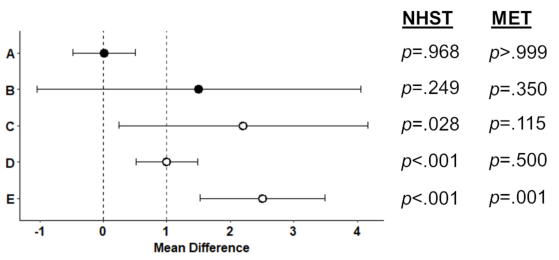
\includegraphics[width=0.8\linewidth]{figs/fig1} 

}

\caption{Figure 1: 95\% confidence intervals and corresponding \emph{p}-values for testing $H_{0}: \Delta = 0$ (NHST, null hypothesis significance testing) and $H_{0}: \Delta \leq 0$ (MET, a one-sided minimal effects test). Open circles indicate mean differences with \emph{p} < 0.05 for the NHST.}\label{fig:fig1pdf}
\end{figure}

Hypothesis testing and estimation cannot be fully disentangled:
estimation (frequentist or Bayesian) asks about \emph{plausible values}
of the parameter in the population, hypothesis testing asks about the
\emph{plausibility of a specific parameter value}. These are both
inferences, because we are inferring something about the population
based on the data in our sample. In the frequentist paradigm,
uncertainty in the inference is accounted for with long-run error
control; e.g., setting the Type 1 Error rate, \(\alpha\) = 0.05. We can
see this when running simulations as shown in Figure 1A-E: any
confidence interval that does not contain zero also has \emph{p}
\textless{} 0.05 for the null hypothesis significance test (NHST).

The 95\% confidence interval shows values in the population that are
\emph{compatible} with what we observed in the sample
(\protect\hyperlink{ref-3}{Rafi \& Greenland, 2020}). That is, if you
move outside of the confidence interval, any of those parameter values
(the ``true'' mean differences; \(\Delta\)'s) would be statistically
different from the mean difference observed in the sample
\((\bar{X}_{d})\) at the \emph{p} \textless{} 0.05 level. Inside of the
confidence interval, none of those parameter values would be
statistically different (p \textgreater{} 0.05) from the observed mean
difference. Recall that the \emph{p}-value is the probability of
observing data as extreme or more extreme, assuming that the null
hypothesis is true, formally written as \(p(\geq\bar{X}_d|H_{0})\).

Typically, the null hypothesis significance test (NHST) assumes that the
true value in the population is 0 (i.e., \(H_{0}:\Delta = 0\)). The
further the sample mean difference is away from 0, the lower the
probability of observing that sample mean, if the null hypothesis were
true. Importantly, the Editorial does not address the fact that we can
set \(H_{0}\) to be any value. For instance, rather than setting
\(H_{0}:\Delta = 0\) (sometimes referred to as the ``nil-hypothesis'')
(\protect\hyperlink{ref-4}{Cohen, 1994}), we can set \(H_{0}\) equal to
any clinically meaningful value of interest. This is referred to as a
minimal effects test (or minimum effect test, MET)
(\protect\hyperlink{ref-5}{Lakens, 2021};
\protect\hyperlink{ref-2}{Murphy \& Myors, 1999}). For the sake of
argument, let's say this value is 1 in Figure 1. Comparing the
confidence intervals to the new null value, you can see that any
confidence intervals that only contain values larger than 1 also have a
\emph{p} \textless{} 0.05 for the minimal effects test (i.e., Figure
1E).\footnote{METs are typically directional, using one-sided hypothesis
  tests (e.g., \(H_{0}: \leq 1\)) whereas NHSTs are often non-
  directional, using two-sided hypothesis tests (e.g.,
  \(H_{0}: \,= 0\)). Thus, although the confidence interval for Figure
  1A does not contain the null value of 1, the whole of the confidence
  interval is below 1, thus yielding a non-significant minimal effects
  test.} Thus, we have both an inference about a specific hypothesis and
an estimate in both the NHST and the MET\footnote{For convenience, I am
  referring to NHST and MET as separate tests. However, it is more
  accurate to think of the MET as a type of NHST where you have a
  one-sided test of a non-zero null value. I use the different terms
  because readers are likely more familiar with the term NHST when
  referring to the specific case of \(H_{0} = 0\)
  (\protect\hyperlink{ref-4}{Cohen, 1994}).}, but the hypothesis test
and the estimate are complementary and connected.

\hypertarget{misleading-arguments-about-flaws-with-significance-tests}{%
\section{Misleading arguments about flaws with significance
tests}\label{misleading-arguments-about-flaws-with-significance-tests}}

The Editorial bases many arguments on a previous list of perceived
problems from Herbert (\protect\hyperlink{ref-6}{2019}). The Herbert
(\protect\hyperlink{ref-6}{2019}) paper is in itself an editorial that
presents informed arguments, but is not an objective demonstration of
any mathematical facts. So, reinforcing the Editorial's list through a
citation to Herbert (\protect\hyperlink{ref-6}{2019}) does not provide
an evidentiary foundation: it is layering opinion on top of opinion.
Second, each of the five ``problems'' outlined by the Editorial is
either not really a problem inherent to \emph{p}-values or the problem
is a true but misleading statement. I address each problem from the
Editorial (in quotes) below:

\textbf{1. ``A \emph{p}-value is not the probability that a hypothesis
is (or is not) true.''} -- This is correct, but it does not follow that
this makes \emph{p}-values, or even statistical significance tests,
unhelpful or uninformative. Knowing that the observed data are
incompatible with some null value is a crucial step for many research
questions. For instance, hypothesis testing in early phase research can
help us make decisions about where to direct our resources, starting us
down the road of replication and ultimately determining the efficacy and
effectiveness of an intervention.

\textbf{2. A \emph{p}-value does not constitute evidence} -- This is an
oversimplification and misleading. The Editorial is correct that a
single \emph{p}-value is not strictly speaking ``evidence'' and cannot
tell us about the probability of the null hypothesis being true.
However, \emph{p}-values are still useful tools for making decisions.

Technical definitions of evidence can get a bit complicated and are
debated (\protect\hyperlink{ref-9}{Goodman \& Royall, 1988};
\protect\hyperlink{ref-7}{Lakens, 2022b}; \protect\hyperlink{ref-8}{Muff
et al., 2022}). However, I would invite readers to consider a simple
example of absolute probability versus relative probability. If I find
that eating green jelly beans reduces post-surgical recovery time for
the ACL by 10\% relative to controls with \emph{p} \textless{} 0.05,
then the most likely explanation is still that jelly beans have no
effect on recovery and what I observed was chance fluctuation. That is,
the null hypothesis is still the most likely explanation even though p
was \textless{} 0.05, because the baseline probability of ``jelly bean
efficacy'' is very low and false positives occur 5\% of the time when
\(\alpha\) = 0.05 . Thus, the \emph{p}-value is not in itself a measure
of evidence, because I would need additional \emph{outside information}
in order to change (or not change) my beliefs. As Goodman \& Royall
(\protect\hyperlink{ref-9}{1988}) write ``The \emph{p}-value is not
adequate for inference because \textbf{\emph{the measurement of
evidence}} requires are least three components: the observations, and
two competing explanations for how they were produced'' (p.~1569;
emphasis added).

Some researchers might think of the \emph{p}-value as evidence against
the null specifically, without the need for comparison to a given
alternative. But the \emph{p}-value is calculated assuming that the null
is true, so again the Editorial is correct that we cannot simply flip
the question around, assume the data, and get the likelihood of the null
being true, i.e., \(p(\bar{x}_{d}|H_{0}) \neq p(H_{0}|\bar{x}_{d})\). To
estimate the likelihood of the null hypothesis being true, we would need
Bayesian statistics in which we formalize some prior probability about
the null hypothesis (\protect\hyperlink{ref-9}{Goodman \& Royall,
1988}). If we have a strong enough prior probability that the null is
true, then the current data in the sample may not lead us to change our
beliefs based on the posterior distribution, no matter how small the
\emph{p}-value. This was the case in my jelly bean example, where
\emph{p} \textless{} 0.05 still did not shake my belief in the null
hypothesis. For any given prior distribution, however, there is a
smaller likelihood of observing highly discrepant effects (e.g.,
\(|\bar{x}_{d}| >> 0\)), leading to a smaller relative probability of 0
in the posterior distribution compared to the prior
distribution.\footnote{For a humorous demonstration see:
  \url{https://xkcd.com/1132/}; for a more quantitative visualization of
  the relationship between priors, \emph{p}-values, and posteriors see:
  \url{https://rpsychologist.com/d3/bayes/}. More technically, the
  posterior (the updated probability density function after we have seen
  the data) is proportional to the prior (our expectation before we saw
  the data) multiplied by the likelihood (which is the probability of
  the current data given the hypothesis):
  \(posterior \propto likelihood \times prior\).} Updating the
probability of 0 in the posterior distribution reflects rational
decision making in daily life. For instance, the first time I find jelly
beans reduce recovery time with \emph{p} \textless{} 0.05, I might
rightly ignore that as a false positive. The fifth time I find jelly
beans reduce recovery time with \emph{p} \textless{} 0.05, I should take
a long hard look at the ingredients and maybe my study procedures; as
\emph{p} \textless{} 0.05 is not always a sign that the null is wrong,
but that some other assumption has been violated.

Still, the \emph{p}-value does not need to be a measure of evidence for
it to be useful. Critically, small \emph{p}-values are relatively less
likely to be observed when the null hypothesis is true compared to when
an alternative hypothesis is true. Thus, in a practical sense, a
\emph{p}-values can help us make decisions about what effects to study,
assuming that we are testing at least some real effects. As shown in
Figure 2A, \emph{p}-values have a uniform distribution under the null
hypothesis, with 5\% of \emph{p}-values necessarily below 0.05. However,
if the null is not true, then we will see a shift in the distribution of
\emph{p}-values, with small \emph{p}-values becoming more common. An
example of this is shown in Figure 2B, where the null is false and 34\%
of \emph{p}-values are below 0.05. However, correctly rejecting the null
hypothesis only 34\% of the time is not ideal, so consider Figure 2C,
where I have now tripled the sample size and 80\% of \emph{p}-values are
below 0.05. That is, with 64 people per group, we now have 80\%
statistical power to detect a \(\Delta = 0.5\).

\begin{figure}[H]

{\centering 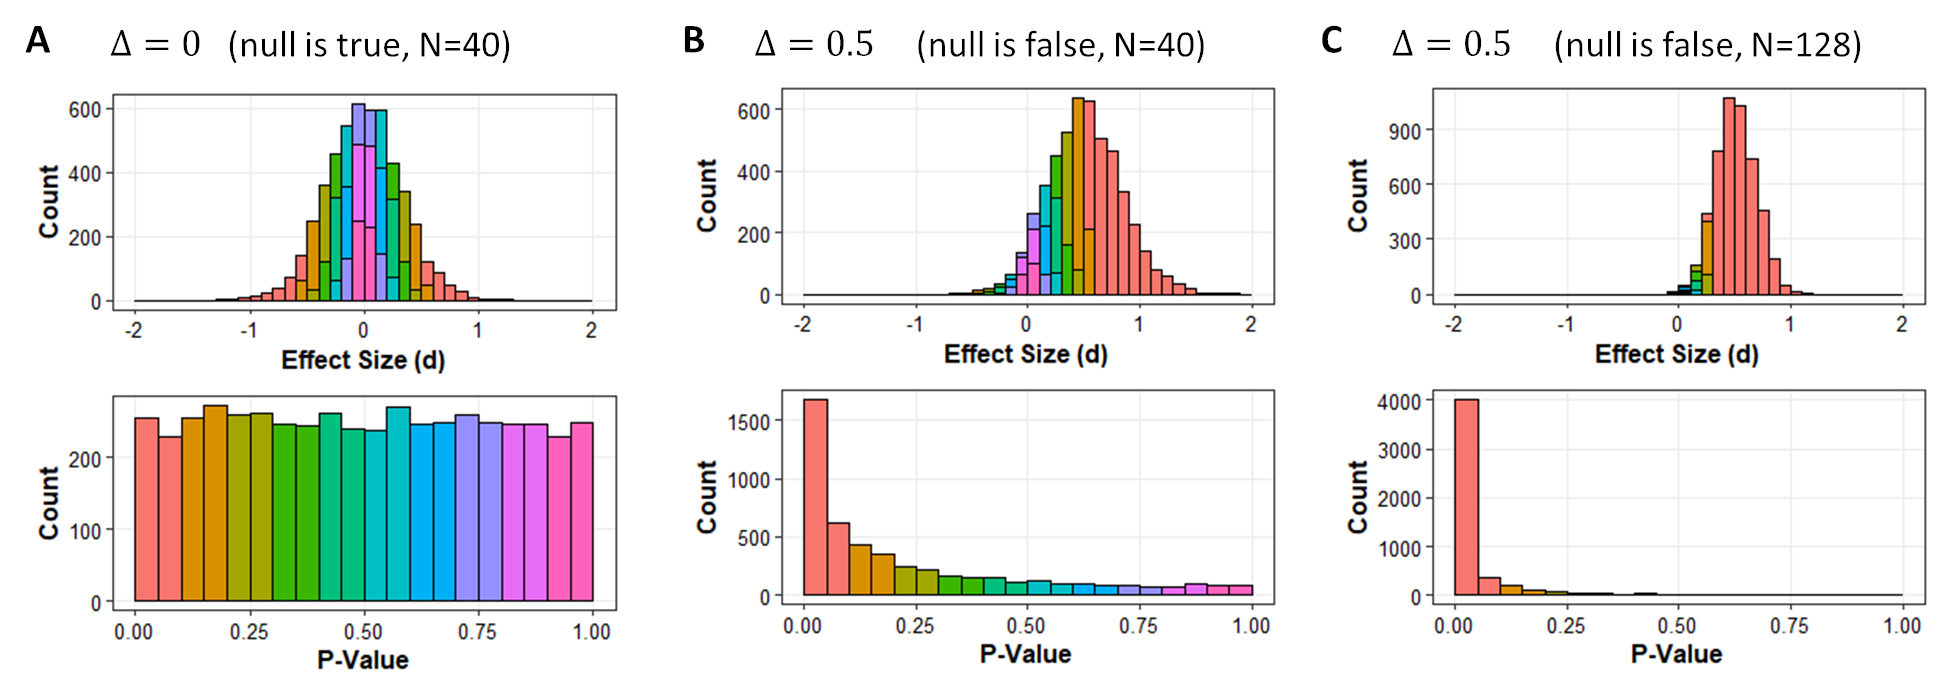
\includegraphics[width=1\linewidth]{figs/fig2} 

}

\caption{Figure 2: \emph{P}-values < 0.05 are more likely to occur when the null is false, and critically will only occur 5\% of the time when the null is true. Plots show simulated experiments ($k$ = 5,000, $\sigma$ = 1 for all populations) in which the means of two independent groups are compared using a t-test. In Panel A, the null hypothesis is true and the true difference between population means is 0. In Panel B, the null hypothesis is false and the true difference between population means is 0.5. In Panel C, the null-hypothesis is still false, but I have increased the sample size from 40 to 128, yielding 80\% of \emph{p}-values < 0.05 (i.e., 80\% statistical power). Quantiles are color coded with respect to their \emph{p}-values and effects sizes are given as Cohen’s $d$.}\label{fig:fig2pdf}
\end{figure}

This is where the concept of a decision is important to distinguish from
the term ``evidence'' (\protect\hyperlink{ref-9}{Goodman \& Royall,
1988}). Without knowing the actual evidence against the null-hypothesis,
if I decide to reject the null when \emph{p} \textless{} 0.05, then I
will only be wrong 5\% of the time (i.e., the Type 1 error rate).
Similarly, if I have 80\% statistical power and a reasonable estimate
for the smallest effect size of interest, then I only have a 20\% chance
of missing an effect of that size (i.e., the Type 2 error rate).
Mathematically, these probabilities are robust if we accept the
null-hypothesis as true and make minimal other assumptions, which is
very helpful when limited outside information is available. See Goodman
quoting Neyman and Pearson about hypothesis testing, ``Without hoping to
know whether each separate hypothesis is true or false, we may search
for rules to govern our behaviour with regard to them, in following
which we insure that, in the long run of experience, we shall not often
be wrong'' (\protect\hyperlink{ref-10}{Goodman, 1999}).

So, \emph{p}-values are not a measure of evidence, but they are useful
tools for helping us make the correct decision. If we want a proper
measure of evidence for one hypothesis versus another, then we can do
more work, but we also need to make more assumptions and/or bring in
outside information. This can be both a feature and bug of \emph{using}
hypothesis tests. We can control long run error rates with minimal
information, but if we do that so habitually that we forget other
information is available, then that is on us not the \emph{p}-value.

\textbf{3. ``Statistically significant findings are not very
replicable.''} -- This is misleading. First, it is difficult to
precisely define replication (\protect\hyperlink{ref-11}{Open Science
Collaboration, 2015}; \protect\hyperlink{ref-12}{Patil et al., 2016}),
but if we think about ``being replicable'' as the probability that a
statistically significant result represents a real, non-zero effect then
we would expect more statistically significant findings to ``replicate''
provided that hypothesis tests have adequate statistical power,
researchers have not engaged in \emph{p}-hacking, there is not selective
reporting of results, etc. Thus, not all statistically significant
findings will replicate (\protect\hyperlink{ref-13}{Scheel et al.,
2021}), but statistically significant findings in well-designed studies
are more likely to replicate (\protect\hyperlink{ref-15}{Anderson \&
Maxwell, 2017}; \protect\hyperlink{ref-14}{Ioannidis, 2005};
\protect\hyperlink{ref-16}{Nosek et al., 2022}). Second and by any
definition, threats to replicability are also going to affect confidence
intervals (the Editorial's proposed solution) as much as they affect
\emph{p}-values, because, again, the \emph{p}-value is intrinsically
linked to the confidence interval. Thus, the Editorial is correct in a
practical sense: many statistically significant findings in the current
literature do not replicate. However, a lack of replication is the fault
of poor study design and questionable research practices, not the use of
hypothesis tests as a method of inference.

\textbf{4. ``In most clinical trials, the null hypothesis must be
false.''} -- This is arguably true but very misleading. It is true that
real treatment effects are unlikely to be precisely 0 (e.g., they might
be +0.001), but it raises the question: Do we really care if the true
effect is 0 or 0.001? And will we ever have the statistical precision to
discern that difference? All measurement has some error, so I would
argue that many effects are functionally 0 even if the (unknowable) true
value is not actually zero. But, in a strict mathematical sense I will
concede the Editorial is correct, if we accept a hyper-precise
definition, the null-hypothesis of \(H_{0}: \Delta = 0.\overline{00}\)
will usually be false. However, if we accept that definition, then all
point-estimates are false and no value will ever be precisely the
minimum clinically important difference either, which is the Editorial's
proposed point-estimate in their alternative.

In response (\protect\hyperlink{ref-17}{2022}) to an independent
critique by Lakens (\protect\hyperlink{ref-18}{2022a}), this
hyper-precise definition does seem to be the argument that the editorial
is making.\footnote{I was very excited to see the Lakens
  (\protect\hyperlink{ref-18}{2022a}) commentary and others
  (\protect\hyperlink{ref-19}{Tenan \& Caldwell, 2022}), and even more
  excited to see we all largely agree. Interestingly, however, I only
  became aware of these commentaries after writing my own because I did
  not see the editorial until it was re-published in Physical Therapy
  (\protect\hyperlink{ref-1}{2022}) in June, 2022, whereas my more
  astute colleagues responded to the original publication in the Journal
  of Physiotherapy (\protect\hyperlink{ref-20}{Elkins et al., 2022}), in
  January 2022. The editorial has been re-published in four different
  journals to date. While I can appreciate trying to spread one's
  message, this creates confusion.} They claim, ``The assertion that the
null hypothesis is false in most clinical trials does not require
empirical evidence, because it is self-evidently true'' and ``The null
hypothesis may often be approximately true, but it is rarely if ever
exactly true''. The Editorial seems to miss the point that the null is a
useful model: testing against 0 is still useful for things that are
approximately 0. As an analogy, I have successfully found my way many
places using maps, but none of those maps was a photo-realistic version
of reality.

Scientists are often working on the frontiers of human knowledge; this
is costly work where we need to explore a lot of different ideas and
many them do not pan out. That is, many tested ``effects'' are
functionally zero (\protect\hyperlink{ref-14}{Ioannidis, 2005}). So,
simply because a point estimate of precisely 0 is unlikely to be true
does not mean that it is unhelpful to ask. It should be a very low bar
to show that your clinical treatment has a non-zero effect! Further, the
Editorial is specifically critiquing this ``nil'' hypothesis (i.e.,
\(H_{0} = 0\)), when we could hypothesize any value, or avoid the
point-null entirely with a one-sided test (i.e., \(H_{0} \leq 0\))
(\protect\hyperlink{ref-5}{Lakens, 2021};
\protect\hyperlink{ref-2}{Murphy \& Myors, 1999}). So, if assuming
\(H_{0} = 0\) is not desirable, we can set that null value to be
anything we want (i.e., \(H_{0}: \Delta \leq 0.4\) m/s for improvement
in gait speed, \(H_{0}: \Delta \leq 30\)\% change on a pain scale, or
\(H_{0}: \Delta \leq 1\) in the hypothetical example in Figure 1).

\textbf{5. ``Researchers need information about the size of effects.''}
-- This is a true statement, but it is not a problem with
\emph{p}-values nor null hypothesis significance tests. To my knowledge,
no statistician has ever recommended that applied researchers ignore
measures of effect size (either raw or standardized). Estimates of
effect size are integral to any results section. I would even take this
one step further and encourage authors to share their data whenever
possible (\protect\hyperlink{ref-21}{Borg, Bon, et al., 2020}), enabling
other researchers to calculate their own effect sizes as there can be
limitations with and confusion about standardized effects sizes, and
there is no one-size-fits-all solution to effect sizes
(\protect\hyperlink{ref-22}{Caldwell \& Vigotsky, 2020};
\protect\hyperlink{ref-24}{Levine \& Hullett, 2002};
\protect\hyperlink{ref-23}{McGrath \& Meyer, 2006}).

\hypertarget{the-editorials-alternative-is-a-hypothesis-test-the-minimal-effects-test}{%
\section{The Editorial's ``alternative'' is a hypothesis test -- the
Minimal Effects
Test}\label{the-editorials-alternative-is-a-hypothesis-test-the-minimal-effects-test}}

After detailing the potential problems with the NHST, the Editorial
proposes an alternative solution in which they encourage authors to
compare their 95\% confidence interval to some minimum clinically
meaningful value (which I will write as \(\delta\)).\footnote{I caution
  that it is difficult to find a single measure of \(\delta\); it
  changes as a function of the study population, the study context, and
  has its own uncertainty due to sampling error
  (\protect\hyperlink{ref-25}{Dabija \& Jain, 2019};
  \protect\hyperlink{ref-19}{Tenan \& Caldwell, 2022}).} Estimation is a
good practice and I would encourage researchers to report 95\%
confidence intervals and interpret their upper and lower limits in
context, when appropriate. However, what the Editorial is suggesting is
effectively an MET where \(H_{0}: \Delta \leq \delta\). That is, if the
test is to see if the 95\% confidence interval does not contain
\(\delta\), then that is mathematically equivalent to an MET assuming
\(H_{0}: \Delta \leq \delta\) and finding \emph{p} \textless{} 0.025.
Note \emph{p} \textless{} 0.025, not \emph{p} \textless{} 0.05, because
most METs are one-sided hypothesis tests whereas confidence intervals
are two sided (see Figure 1 and Footnote 1). After heavily critiquing
hypothesis testing as a method of inference, the Editorial ends up
effectively proposing a hypothesis test. This is clearly an illogical
proposition.

I want to emphasize that it is valid for the Editorial to recommend that
authors consider their 95\% confidence interval relative to some
clinically meaningful value. However, this is not an ``alternative'' to
conducting a null hypothesis significance test, it is in fact
mathematically identical to conducting a null hypothesis test with a
carefully chosen null hypothesis. Both are valid.

I would add, however, that there are also advantages to explicitly
framing this as a hypothesis test rather than the informal
interpretation of a confidence interval. First, it encourages
researchers to explicitly commit to a specific \(\delta\) while the
study is being designed, rather than simply obtaining an estimate of the
effect and then comparing it to candidate \(\delta\)'s post hoc. Second,
it requires researchers to think carefully about the direction of the
test and the desired \(\alpha\)-level, whereas simply invoking a 95\%
confidence interval implicitly uses a two-tailed test and
\(\alpha = 0.05\), which may not be best suited to the research
question.

Finally, it is also important to stress that history provides us with
several examples of how authors will view their data through rose-tinted
glasses when quantitative statistical safeguards are removed. For
instance, when \emph{Basic and Applied Social Psychology} banned
\emph{p}-values, authors were found to overstate their conclusions well
beyond what would have been considered if ``statistical significance''
had been a benchmark (\protect\hyperlink{ref-26}{Fricker Jr. et al.,
2019}). In sport and exercise science, ``magnitude-based inference'' was
leveraged as a niche method that allowed authors to interpret
differences as meaningful when they had very little statistical support
(e.g., \emph{p}'s \textgreater{} 0.25) (\protect\hyperlink{ref-29}{Lohse
et al., 2020}; \protect\hyperlink{ref-27}{Sainani, 2018};
\protect\hyperlink{ref-28}{Sainani et al., 2019}). Statistical
significance in an NHST does not necessarily need to be the benchmark
nor 0.05 the default value (\protect\hyperlink{ref-32}{Amrhein \&
Greenland, 2018}; \protect\hyperlink{ref-30}{Benjamin et al., 2018};
\protect\hyperlink{ref-31}{Lakens et al., 2018};
\protect\hyperlink{ref-33}{McShane et al., 2019}), but it is always
important to have a statistically sound framework for dealing with
uncertainty.

\hypertarget{virtues-of-hypothesis-testing}{%
\section{Virtues of hypothesis
testing}\label{virtues-of-hypothesis-testing}}

One of the great virtues of null hypothesis significance testing is Type
I error control while making minimal assumptions about the nature of the
data or the world at large. If we set \(\alpha = 0.05\), then we can be
confident we will only get data greater than or equal to what we
observed 5\% of the time when the null is true. Importantly, this works
for a wide range of statistics and types of tests, including \emph{F}-
and \(\chi^2\)-statistics that have multiple degrees of freedom from
models asking questions about multiple effects simultaneously. For
instance, in a randomized controlled trial with three arms, I could
conduct an omnibus \emph{F}-test and obtain a \emph{p}-value to see if
there is any evidence of a difference between groups overall, before
conducting additional post-hoc tests to compare specific groups. This
situation is not covered by the Editorial and the Editorial's confidence
interval alternative is not easily applied here, although one could
plausibly adjust the width of the confidence intervals to control for
multiple comparisons.

\hypertarget{bigger-threats-to-statistical-integrity}{%
\section{Bigger threats to statistical
integrity}\label{bigger-threats-to-statistical-integrity}}

Misinterpretation and misuse of \emph{p}-values are threats to
statistical integrity. However, questionable research practices such as
\emph{p}-hacking, sub-group analyses, flexible stopping rules, selective
exclusion of outliers, selective reporting, and hypothesizing after
results are known (HARKing) are much larger threats
(\protect\hyperlink{ref-37}{Kerr, 1998};
\protect\hyperlink{ref-38}{Rosenthal, 1979};
\protect\hyperlink{ref-35}{Simmons et al., 2011},
\protect\hyperlink{ref-34}{2013}; \protect\hyperlink{ref-36}{Sun et al.,
2012}). Furthermore, these questionable research practices have
consistently negative consequences regardless of the method of
inference. For instance, although the term ``\emph{p}-hacking'' connotes
the NHST, these questionable research practices pose an equal threat to
confidence intervals because again confidence intervals and
\emph{p}-values are based on the same underlying mathematics. Similarly,
switching to a fully Bayesian method of analysis is not an antidote for
poor study design, small samples, and questionable research practices.
As others have argued (\protect\hyperlink{ref-39}{Borg, Lohse, et al.,
2020}; \protect\hyperlink{ref-40}{Leek \& Peng, 2015}), \emph{p}-values
get a disproportionate amount of attention in popular discussions of
research methodology. I encourage the ISPJE to instead focus their
attention on methods for improving data/code sharing, transparency, and
replicability through tools like preregistration, results-blind review,
registered reports, or even ``data papers'' whose primary function is to
report a study and archive the data, without drawing inferences from
limited samples.

It is entirely valid to say that \emph{p}-values are often mis-used and
mis-interpreted, and ``statistical significance'' may not ultimately be
the best term for applied researchers to use
(\protect\hyperlink{ref-41}{Wasserstein et al., 2019}). However, it is
incorrect to present these human errors as inherent flaws in hypothesis
testing. For instance, if someone mis-interprets p \textgreater{} 0.05
as evidence of ``no difference'', then I would argue the correct action
is to teach them about equivalence tests and non-inferiority designs,
not ban \emph{p}-values. Similarly, there are times when Bayesian
inference is what authors are really interested in (e.g., what is the
probability that the null is true, given the evidence?), and in those
cases Bayesian inference can and should be used. However, Bayesian
analysis is not a panacea and needs to be used thoughtfully like any
statistical tool. So, although a simple heuristic of \emph{p}
\textless{} 0.05 may well be overused as ``the'' test in physical
therapy research, frequentist hypothesis tests are still valid and
useful tools for physical therapy researchers. Moreover, the scientific
integrity of the field has much larger concerns, and both
\emph{p}-values and confidence intervals will be corrupted by
\emph{p}-hacking, under-powered subgroup analyses, surrogate outcomes,
and other questionable research practices.

In conclusion, I agree with the Editorial on the importance of reporting
effect sizes and interpreting them in context. However, the Editorial
makes numerous statistical \emph{faux pas} that could harm the
statistical literacy in our field, if readers take them at face value,
and harm the scientific integrity of our field, if put into editorial
practice.

\newpage

\hypertarget{additional-information}{%
\section{Additional Information}\label{additional-information}}

\hypertarget{data-accessibility}{%
\subsection{Data Accessibility}\label{data-accessibility}}

\texttt{R} code for all analyses and simulations presented in this
commentary are included as a digital supplement on SportRxiv
(\url{https://sportrxiv.org/index.php/server/preprint/view/178/version/211}).

\hypertarget{conflict-of-interest}{%
\subsection{Conflict of Interest}\label{conflict-of-interest}}

Author has no conflicts of interest to declare.

\hypertarget{funding}{%
\subsection{Funding}\label{funding}}

None.

\hypertarget{acknowledgments}{%
\subsection{Acknowledgments}\label{acknowledgments}}

I would like to thank Dr.~Emma Johnson, Dr.~Kristin Sainani, and two
anonymous reviewers for their detailed comments on earlier drafts of
this commentary.

\hypertarget{preprint}{%
\subsection{Preprint}\label{preprint}}

The pre-publication version of this manuscript can be found on SportRxiv
(DOI: \url{https://doi.org/10.51224/SRXIV.178}).

\newpage

\hypertarget{references}{%
\section{References}\label{references}}

\parindent0pt 
\setlength{\parskip}{1em}

\hypertarget{refs}{}
\begin{CSLReferences}{1}{0}
\leavevmode\vadjust pre{\hypertarget{ref-32}{}}%
Amrhein, V., \& Greenland, S. (2018). Remove, rather than redefine,
statistical significance. \emph{Nature Human Behavior}, \emph{2}, 4--4.
\url{https://doi.org/10.1038/s41562-017-0224-0}

\leavevmode\vadjust pre{\hypertarget{ref-15}{}}%
Anderson, S. F., \& Maxwell, S. E. (2017). Addressing the {``replication
crisis''}: Using original studies to design replication studies with
appropriate statistical power. \emph{Multivariate Behavioral Research},
\emph{52}, 305--324. \url{https://doi.org/10.1080/00273171.2017.1289361}

\leavevmode\vadjust pre{\hypertarget{ref-30}{}}%
Benjamin, D. J., Berger, J. O., Johannesson, M., Nosek, B. A.,
Wagenmakers, E. J., Berk, R., ..., \& Johnson, V. E. (2018). Redefine
statistical significance. \emph{Nature Human Behavior}, \emph{2}, 6--10.
\url{https://doi.org/10.1038/s41562-017-0189-z}

\leavevmode\vadjust pre{\hypertarget{ref-21}{}}%
Borg, D. N., Bon, J., Sainani, K. L., Baguley, B. J., Tierney, N., \&
Drovandi, C. (2020). Sharing data and code: A comment on the call for
the adoption of more transparent research practices in sport and
exercise science. \emph{SportRxiv}.
\url{https://doi.org/10.31236/osf.io/ftdgj}

\leavevmode\vadjust pre{\hypertarget{ref-39}{}}%
Borg, D. N., Lohse, K. R., \& Sainani, K. L. (2020). Ten common
statistical errors from all phases of research, and their fixes.
\emph{PM\&R}, \emph{12}, 610--614.
\url{https://doi.org/10.1002/pmrj.12395}

\leavevmode\vadjust pre{\hypertarget{ref-22}{}}%
Caldwell, A., \& Vigotsky, A. D. (2020). A case against default effect
sizes in sport and exercise science. \emph{PeerJ}, \emph{8, e10314}.
\url{https://doi.org/10.7717/peerj.10314}

\leavevmode\vadjust pre{\hypertarget{ref-4}{}}%
Cohen, J. (1994). The earth is round (p \textless{} .05). \emph{American
Psychologist}, \emph{49}, 997--1003.
\url{https://doi.org/10.1037/0003-066X.49.12.997}

\leavevmode\vadjust pre{\hypertarget{ref-25}{}}%
Dabija, D. I., \& Jain, N. B. (2019). Minimal clinically important
difference of shoulder outcome measures and diagnoses: A systematic
review. \emph{American Journal of Physical Medicine \& Rehabilitation},
\emph{98}, 671--676. \url{https://doi.org/10.1097/phm.0000000000001169}

\leavevmode\vadjust pre{\hypertarget{ref-1}{}}%
Elkins, M. R., Pinto, R. Z., Verhagen, A., Grygorowicz, M., Soderlund,
A., Guemann, M., Gomez-Conesa, A., Blanton, S., Brismée, J. M., Agarwal,
S., Jette, A., Karstens, S., Harms, M., Verheyden, G., \& Sheikh, U.
(2022). Statistical inference through estimation: Recommendations from
the International Society of Physiotherapy Journal Editors.
\emph{Physical Therapy}, \emph{102}, pzac066.
\url{https://doi.org/10.1016/j.jphys.2021.12.001}

\leavevmode\vadjust pre{\hypertarget{ref-17}{}}%
Elkins, M. R., Pinto, R. Z., Verhagen, A., Grygorowicz, M., Söderlund,
A., Guemann, M., Gómez-Conesa, A., Blanton, S., Brismée, J. M., Agarwal,
S., Jette, A., Harms, M., Verheyden, G., \& Sheikh, U. (2022).
Correspondence: Response to Lakens. \emph{Journal of Physiotherapy},
\emph{68}, 214. \url{https://doi.org/10.1016/j.jphys.2022.06.003}

\leavevmode\vadjust pre{\hypertarget{ref-20}{}}%
Elkins, M. R., Pinto, R. Z., Verhagen, A., Grygorowicz, M., Söderlund,
A., Guemann, M., Gómez-Conesa, A., Blanton, S., Brismée, J. M., Ardern,
C., Agarwal, S., Jette, A., Karstens, S., Harms, M., Verheyden, G., \&
Sheikh, U. (2022). Statistical inference through estimation:
Recommendations from the International Society of Physiotherapy Journal
Editors. \emph{Journal of Physiotherapy}, \emph{68}(1), 1--4.
\url{https://doi.org/10.1016/j.jphys.2021.12.001}

\leavevmode\vadjust pre{\hypertarget{ref-26}{}}%
Fricker Jr., R. D., Burke, K., Han, X., \& Woodall, W. H. (2019).
Assessing the statistical analyses used in Basic and Applied Social
Psychology after their p-value ban. \emph{The American Statistician},
\emph{73}, 374--384. \url{https://doi.org/10.1080/00031305.2018.1537892}

\leavevmode\vadjust pre{\hypertarget{ref-10}{}}%
Goodman, S. N. (1999). Toward evidence-based medical statistics. 1: The
P value fallacy. \emph{Annals of Internal Medicine,} \emph{130},
995--1004.
\url{https://doi.org/10.7326/0003-4819-130-12-199906150-00008}

\leavevmode\vadjust pre{\hypertarget{ref-9}{}}%
Goodman, S. N., \& Royall, R. (1988). Evidence and scientific research.
\emph{American Journal of Public Health}, \emph{78}, 1568--1574.
\url{https://doi.org/10.2105/ajph.78.12.1568}

\leavevmode\vadjust pre{\hypertarget{ref-6}{}}%
Herbert, R. (2019). Research note: Significance testing and hypothesis
testing: Meaningless, misleading and mostly unnecessary. \emph{Journal
of Physiotherapy}, \emph{65}, 178--181.
\url{https://doi.org/10.1016/j.jphys.2019.05.001}

\leavevmode\vadjust pre{\hypertarget{ref-14}{}}%
Ioannidis, J. P. (2005). Why most published research findings are false.
\emph{PLoS Medicine}, \emph{2, e124}.
\url{https://doi.org/10.1371/journal.pmed.0020124}

\leavevmode\vadjust pre{\hypertarget{ref-37}{}}%
Kerr, N. L. (1998). HARKing: Hypothesizing after the results are known.
\emph{Personality and Social Psychology Review}, \emph{2}, 196--217.
\url{https://doi.org/10.1207/s15327957pspr0203_4}

\leavevmode\vadjust pre{\hypertarget{ref-5}{}}%
Lakens, D. (2021). The practical alternative to the p value is the
correctly used p value. \emph{Perspectives on Psychological Science},
\emph{16}, 639--648. \url{https://doi.org/10.1177/1745691620958012}

\leavevmode\vadjust pre{\hypertarget{ref-18}{}}%
Lakens, D. (2022a). Correspondence: Reward, but do not yet require,
interval hypothesis tests. \emph{Journal of Physiotherapy}, \emph{68},
213--214. \url{https://doi.org/10.1016/j.jphys.2022.06.004}

\leavevmode\vadjust pre{\hypertarget{ref-7}{}}%
Lakens, D. (2022b). Why P values are not measures of evidence.
\emph{Trends in Ecology \& Evolution}, \emph{37}, 289--290.
\url{https://doi.org/10.1016/j.tree.2021.12.006}

\leavevmode\vadjust pre{\hypertarget{ref-31}{}}%
Lakens, D., Adolfi, F. G., Albers, C. J., Anvari, F., Apps, M. A.,
Argamon, S. E., ..., \& Zwaan, R. A. (2018). Justify your alpha.
\emph{Nature Human Behavior}, \emph{2}, 168--171.
\url{https://doi.org/10.1038/s41562-018-0311-x}

\leavevmode\vadjust pre{\hypertarget{ref-40}{}}%
Leek, J. T., \& Peng, R. D. (2015). Statistics: P values are just the
tip of the iceberg. \emph{Nature}, \emph{520}, 612--612.
\url{https://doi.org/10.1038/520612a}

\leavevmode\vadjust pre{\hypertarget{ref-24}{}}%
Levine, T. R., \& Hullett, C. R. (2002). Eta squared, partial eta
squared, and misreporting of effect size in communication research.
\emph{Human Communication Research}, \emph{28}, 612--625.
\url{https://doi.org/10.1111/j.1468-2958.2002.tb00828.x}

\leavevmode\vadjust pre{\hypertarget{ref-29}{}}%
Lohse, K. R., Sainani, K. L., Taylor, A., Butson, M. L., Knight, E. J.,
\& Vickers, A. J. (2020). Systematic review of the use of
{``magnitude-based inference''} in sports science and medicine.
\emph{PLoS One}, \emph{15}, 0235318.
\url{https://doi.org/10.1371/journal.pone.0235318}

\leavevmode\vadjust pre{\hypertarget{ref-23}{}}%
McGrath, R. E., \& Meyer, G. J. (2006). When effect sizes disagree: the
case of r and d. \emph{Psychological Methods}, \emph{11}, 386.
\url{https://doi.org/10.1037/1082-989x.11.4.386}

\leavevmode\vadjust pre{\hypertarget{ref-33}{}}%
McShane, B. B., Gal, D., Gelman, A., Robert, C., \& Tackett, J. L.
(2019). Abandon statistical significance. \emph{The American
Statistician}, \emph{73}, 235--245.
\url{https://doi.org/10.1080/00031305.2018.1527253}

\leavevmode\vadjust pre{\hypertarget{ref-8}{}}%
Muff, S., Nilsen, E. B., O'Hara, R. B., \& Nater, C. R. (2022). Response
to {``Why P values are not measures of evidence''} by D. Lakens.
\emph{Trends in Ecology \& Evolution}, \emph{37}, 291--292.
\url{https://doi.org/10.1016/j.tree.2022.01.001}

\leavevmode\vadjust pre{\hypertarget{ref-2}{}}%
Murphy, K. R., \& Myors, B. (1999). Testing the hypothesis that
treatments have negligible effects: Minimum-effect tests in the general
linear model. \emph{Journal of Applied Psychology}, \emph{84}, 234--248.
\url{https://doi.org/10.1037/0021-9010.84.2.234}

\leavevmode\vadjust pre{\hypertarget{ref-16}{}}%
Nosek, B. A., Hardwicke, T. E., Moshontz, H., Allard, A., Corker, K. S.,
Dreber, A., Fidler, F., Hilgard, J., Struhl, M. K., Nuijten, M. B.,
Rohrer, J. M., Romero, R., Scheel, A. M., Scherer, L. D., Schönbrodt, B.
A., Nosek, F. D., \& Vazire16, S. (2022). Replicability, robustness, and
reproducibility in psychological science. \emph{Annual Review of
Psychology}, \emph{73}, 719--748.
\url{https://doi.org/10.1146/annurev-psych-020821-114157}

\leavevmode\vadjust pre{\hypertarget{ref-11}{}}%
Open Science Collaboration. (2015). Estimating the reproducibility of
psychological science. \emph{Science}, \emph{349}, 4716.
\url{https://doi.org/10.1126/science.aac4716}

\leavevmode\vadjust pre{\hypertarget{ref-12}{}}%
Patil, P., Peng, R. D., \& Leek, J. T. (2016). What should researchers
expect when they replicate studies? A statistical view of replicability
in psychological science. \emph{Perspectives on Psychological Science},
\emph{11}, 539--544. \url{https://doi.org/10.1177/1745691616646366}

\leavevmode\vadjust pre{\hypertarget{ref-3}{}}%
Rafi, Z., \& Greenland, S. (2020). Semantic and cognitive tools to aid
statistical science: replace confidence and significance by
compatibility and surprise. \emph{BMC Medical Research Methodology},
\emph{20}, 244. \url{https://doi.org/10.1186/s12874-020-01105-9}

\leavevmode\vadjust pre{\hypertarget{ref-38}{}}%
Rosenthal, R. (1979). The file drawer problem and tolerance for null
results. \emph{Psychological Bulletin}, \emph{86}.
\url{https://doi.org/10.1037/0033-2909.86.3.638}

\leavevmode\vadjust pre{\hypertarget{ref-27}{}}%
Sainani, K. L. (2018). The Problem with {``Magnitude-based Inference.''}
\emph{Medicine and Science in Sports and Exercise}, \emph{50},
2166--2176. \url{https://doi.org/10.1249/mss.0000000000001645}

\leavevmode\vadjust pre{\hypertarget{ref-28}{}}%
Sainani, K. L., Lohse, K. R., Jones, P. R., \& Vickers, A. (2019).
Magnitude‐based inference is not Bayesian and is not a valid method of
inference. \emph{Scandinavian Journal of Medicine \& Science in Sports},
\emph{29}, 1428. \url{https://doi.org/10.1111/sms.13491}

\leavevmode\vadjust pre{\hypertarget{ref-13}{}}%
Scheel, A. M., Schijen, M. R. M. J., \& Lakens, D. (2021). An excess of
positive results: Comparing the standard Psychology literature with
Registered Reports. \emph{Advances in Methods and Practices in
Psychological Science}, \emph{4}, 25152459211007468.
\url{https://doi.org/10.1177/25152459211007467}

\leavevmode\vadjust pre{\hypertarget{ref-35}{}}%
Simmons, J. P., Nelson, L. D., \& Simonsohn, U. (2011). False-positive
psychology: Undisclosed flexibility in data collection and analysis
allows presenting anything as significant. \emph{Psychological Science},
\emph{22, 11}, 1359--1366.
\url{https://doi.org/10.1177/0956797611417632}

\leavevmode\vadjust pre{\hypertarget{ref-34}{}}%
Simmons, J. P., Nelson, L. D., \& Simonsohn, U. (2013). Life after
p-hacking. \emph{Meeting of the Society for Personality and Social
Psychology}, 17--19. \url{https://dx.doi.org/10.2139/ssrn.2205186}

\leavevmode\vadjust pre{\hypertarget{ref-36}{}}%
Sun, X., Briel, M., Busse, J. W., You, J. J., Akl, E. A., Mejza, F.,
..., \& Guyatt, G. H. (2012). Credibility of claims of subgroup effects
in randomised controlled trials: Systematic review. \emph{BMJ},
\emph{344}. \url{https://doi.org/10.1136/bmj.e1553}

\leavevmode\vadjust pre{\hypertarget{ref-19}{}}%
Tenan, M. S., \& Caldwell, A. R. (2022). Confidence intervals and
smallest worthwhile change are not a panacea: A response to the
International Society of Physiotherapy Journal Editors.
\emph{Communications in Kinesiology}, \emph{1, 4}, 1--10.
\url{https://doi.org/10.51224/cik.2022.45}

\leavevmode\vadjust pre{\hypertarget{ref-41}{}}%
Wasserstein, R. L., Schirm, A. L., \& Lazar, N. A. (2019). Moving to a
world beyond {``p\textless{} 0.05.''} \emph{The American Statistician},
\emph{73}, 1--19. \url{https://doi.org/10.1080/00031305.2019.1583913}

\end{CSLReferences}

%
%
%\aucontribute{}

%
%
%
%


\end{document}
